%%%%%%%%%%%%%%%%%%%%%%%%%%%%%%%%%%%%%%%%%%%%%%%%%%%%%%%%%%%%%%%%%%%%%%%%%%%%%%
\documentclass{beamer}            % Generate slides
%\documentclass[handout]{beamer}   % Generate handouts (6 slides to 1 page)
%\documentclass[aspectratio=169]{beamer}  % Use widescreen 16:9 aspect ratio
    % Possible aspect ratios are 16:9, 16:10, 14:9, 5:4, 4:3 (default) and 3:2
    % (Remember to remove the colon)

\usetheme{UoB}
%\usetheme[compress]{UoB}     % Compress the margins
%\usetheme[nourl]{UoB}        % Remove the footer with the URL
%\usetheme[nowatermark]{UoB}  % Remove the watermark from the title page

% Generate handouts with notes (3 slides + 3 notes to 1 page)
%\mode<handout>{
%  \pgfpagesuselayout{3 on 1 with notes}[a4paper,border shrink=10mm]
%}

\usepackage{graphicx}
\usepackage{framed}
\usepackage{multirow}
\usepackage{algorithm}
\usepackage{animate}
%\usepackage{algorithmic}
\usepackage[export]{adjustbox}
\usepackage{algpseudocode}
\usepackage{ulem}
\newcommand\textline[4][t]{%
  \par\smallskip\noindent\parbox[#1]{.116666\textwidth}{\raggedright #2}%
  \parbox[#1]{.666666\textwidth}{\centering#3}%
  \parbox[#1]{.166666\textwidth}{\raggedleft\texttt{#4}}\par\smallskip%
}

%%%%%%%%%%%%%%%%%%%%%%%%%%%%%%%%%%%%%%%%%%%%%%%%%%%%%%%%%%%%%%%%%%%%%%%%%%%%%%
\title[]{Standard Lattice-Based Key Encapsulation on Embedded Devices}
%\subtitle{Subtitle}
\author{\underline{James Howe}$^\dagger$, Tobias Oder$^\ddagger$, Markus Krausz$^\ddagger$, and Tim G\"uneysu$^{\ddagger *}$.}
\institute{$^\dagger$University of Bristol, UK; $^\ddagger$Ruhr-Universit\"at Bochum, Germany;\\ and $^{*}$DFKI, Germany.}
\date{11 September 2018}
%\date{28$^\text{th}$ May 2018}

%%%%%%%%%%%%%%%%%%%%%%%%%%%%%%%%%%%%%%%%%%%%%%%%%%%%%%%%%%%%%%%%%%%%%%%%%%%%%%
\begin{document}

\titlepage

%%%%%%%%%%%%%%%%%%%%%%%%%%%%%%%%%%%%%%%%%%%%%%%%%%%%%%%%%%%%
\begin{frame}{Outline}

\begin{minipage}{0.64\textwidth}
  \begin{itemize}%[<+->]
\item Motivation
\item \sout{Post-quantum cryptography and LWE}
\item Introduction to Frodo  
\item Microcontroller design
\item Hardware design
\item Results and performance analysis
%\item Future research
  \end{itemize}
\end{minipage}
\begin{minipage}{0.35\textwidth}
    %\rule{\textwidth}{0.75\textwidth}
    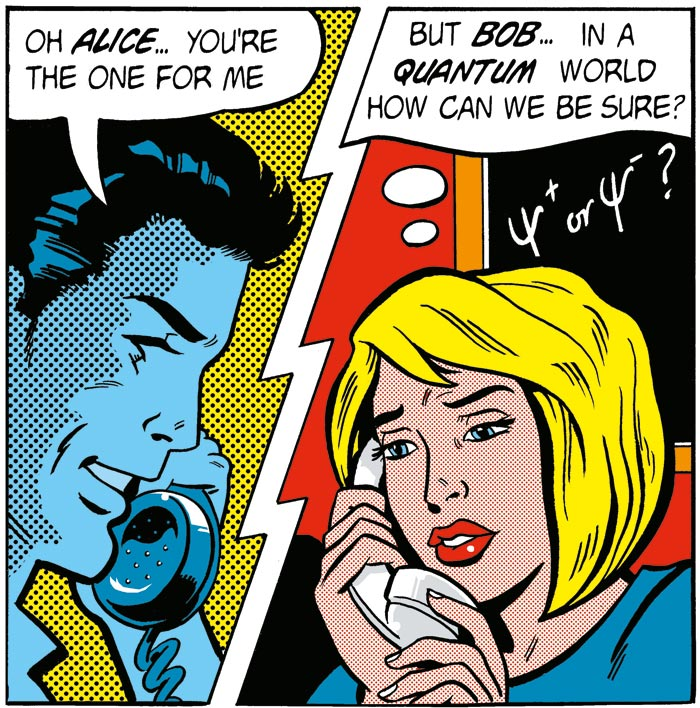
\includegraphics[scale=0.16]{quantumalice}
\end{minipage}  

\end{frame}

%%%%%%%%%%%%%%%%%%%%%%%%%%%%%%%%%%%%%%%%%%%%%%%%%%%%%%%%%%%%%
%\begin{frame}{Motivation}
%
%  \begin{itemize}%[<+->]
%\item What happens when quantum computers become a reality 10-15 years from now?​
%
%\item Commonly used public-key cryptographic algorithms (based on integer factorization and discrete log problem) such as:​
%
%\begin{center}
%\centering
%\textbf{RSA, DSA, Diffie-Hellman Key Exchange, ECC, ECDSA} ​
%\end{center}
%
%will be vulnerable to Shor's algorithm and will no longer be secure.​
%
%  \begin{itemize}
%  \scriptsize
%  \item[]
%\item[]
%\item ``Worse than Y2K: quantum computing and the end of privacy'' -- \emph{Forbes}, 2018.
%\item ``The quantum clock is ticking on encryption - and your data is under threat​'' -- \emph{Wired}, 2016.
%\item ``Unbreakable: The race to protect our secrets from quantum hacks'' -- \emph{New Scientist}, 2018.
%  \end{itemize}
%  \end{itemize}
%
%\end{frame}

%%%%%%%%%%%%%%%%%%%%%%%%%%%%%%%%%%%%%%%%%%%%%%%%%%%%%%%%%%%%
%\begin{frame}{Motivation}
%
%\begin{itemize}[<+->]
%  
%\item Quantum computers exploit the power of parallelism.
%\begin{itemize}
%%\item<.-> Quantum computers break ECC and RSA.
%\item<.-> Classically hard computational problems are now trivial.
%%\item<.-> Governments and companies in preparation.
%\end{itemize}
%\end{itemize}
%
%\begin{minipage}{0.67\textwidth}
%\begin{itemize}[<+->]
%
%
%\item<+-> Shor's Algorithm (1994)
%\begin{itemize}
%\item<.-> Can quickly factorise large numbers (exponential speed-up).
%\item<.-> Significant implications for current public-key cryptography.
%\end{itemize}
%
%\item<+-> Grover's Algorithm (1996)
%\begin{itemize}
%\item<.-> Can search an unsorted database faster than a conventional computer, effects symmetric-key cryptography, so AES-128 now 64-bit secure.
%\end{itemize}
%
%\end{itemize}
%
%\end{minipage}
%\begin{minipage}{0.3\textwidth}
%\begin{framed} \centering
%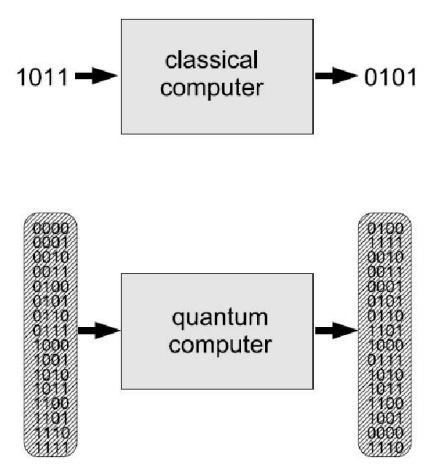
\includegraphics[scale=0.16]{quantum-comp.png}
%\end{framed}
%\end{minipage}  
%
%\end{frame}

%%%%%%%%%%%%%%%%%%%%%%%%%%%%%%%%%%%%%%%%%%%%%%%%%%%%%%%%%%%%
\begin{frame}{Motivation}

\begin{itemize}
\item NIST have started a post-quantum standardisation ``competition''.

\item The call suggests future rounds will likely involve:
\begin{itemize}
\item<.-> Evaluations on constrained devices, such as smart cards,
\item<.-> as well as comparisons of the schemes in hardware.
\end{itemize}
\end{itemize}

\begin{minipage}{0.67\textwidth}
\begin{itemize}

\item Why focus on lattice-based / Frodo?
\begin{itemize}
\item<.-> Extremely versatile and theoretically sound.
\item<.-> Probably the most secure lattice candidate.
\item<.-> Less implementations than ideal lattice schemes; has larger keys and no NTT.
\item<.-> Frodo is ideal for long-term security \emph{and} constrained (hardware) platforms.
\end{itemize}

\end{itemize}

\end{minipage}
\begin{minipage}{0.3\textwidth}
\begin{flushright}
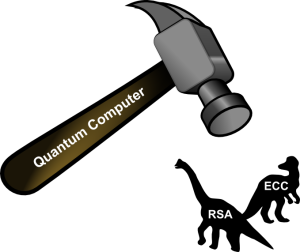
\includegraphics[scale=0.46]{qc-300x252}
\end{flushright}
\end{minipage}  

%NIST welcomes comments regarding the efficiency of the submitted algorithms when implemented in hardware. During the second evaluation period, NIST may request specifications of some of the algorithms using a hardware description language, to compare the estimated hardware efficiency of the submitted algorithms. 

\end{frame}

%%%%%%%%%%%%%%%%%%%%%%%%%%%%%%%%%%%%%%%%%%%%%%%%%%%%%%%%%%%%%
%\begin{frame}{Frodo: Take off the ring!}
%%\newcommand{\Mod}[1]{\ \mathrm{mod}\ #1}
%
%\begin{quote}
%The \textsf{FrodoKEM} schemes are designed to be conservative yet practical post-quantum constructions whose
%security derives from cautious parameterizations of the well-studied learning with errors problem, which in
%turn has close connections to conjectured-hard problems on generic, “algebraically unstructured” lattices.
%\end{quote}
%
%\end{frame}

%%%%%%%%%%%%%%%%%%%%%%%%%%%%%%%%%%%%%%%%%%%%%%%%%%%%%%%%%%%%

\begin{frame}{Frodo: Take off the ring!}

The design philosophy of \textsf{FrodoKEM}~\cite{frodo-nist} combines:

\begin{itemize}[<+->]
\item<.-> Conservative yet practical post-quantum constructions.

\item<.-> Security derived from cautious parameterizations of the well-studied learning with errors problem. 

\item<.-> Thus, close connections to conjectured-hard problems on generic, ``algebraically unstructured'' lattices.

\item Parameter selection is far less constrained than vs ideal lattice schemes.

\end{itemize}

\end{frame}

%%%%%%%%%%%%%%%%%%%%%%%%%%%%%%%%%%%%%%%%%%%%%%%%%%%%%%%%%%%%

\begin{frame}{Frodo: Why should we take off the ring?}

These qualities are appealing for practitioners;

\begin{itemize}[<+->]
\item<.-> Many IoT use cases require long-term, efficient cryptography.

\item<.-> Post-quantum cryptography is becoming essential.

\item<.-> Microcontrollers and FPGAs will play a role in future technologies.

\item<.-> Suitable for use cases such as satellite communications and V2X.

\end{itemize}

\end{frame}

%%%%%%%%%%%%%%%%%%%%%%%%%%%%%%%%%%%%%%%%%%%%%%%%%%%%%%%%%%%%

%\begin{frame}{Frodo: KEM from standard lattices}
%
%\begin{center}
%
%\begin{algorithm}[H]
%\centering
%\footnotesize
%\caption{The \textsf{FrodoKEM} decapsulation (shortened)} \label{alg:decaps}
%  \begin{algorithmic}
%\footnotesize
%    \Procedure{Decaps}{$sk=(\mathbf{s} || \text{seed}_\mathbf{A} || \mathbf{B}, \mathbf{S}),\mathbf{c}_1 || \mathbf{c}_2 || \mathbf{d}$}
%	 %\State Compute $\mathbf{B}^\prime \leftarrow \text{Frodo.Unpack}(\mathbf{c}_1)$
%	 %\State Compute $\mathbf{C} \leftarrow \text{Frodo.Unpack}(\mathbf{c}_2)$
%	 \State Compute $\mathbf{M} \leftarrow \mathbf{C} - \mathbf{B}^\prime \mathbf{S}$	
%	 \State Compute $\mu^\prime \leftarrow \text{Frodo.Decode}(\mathbf{M})$	 
%	 %\State Parse $pk \leftarrow \text{seed}_\mathbf{A} || \mathbf{b}$
%	 \State Generate pseudo-random values $\text{seed}^\prime_\mathbf{E} || \mathbf{k}^\prime || \mathbf{d}^\prime \leftarrow G(pk || \mu^\prime)$
%	 
%	\State Sample error matrix $\mathbf{S}^\prime ,\mathbf{E}^\prime \leftarrow \text{Frodo.SampleMatrix}(\text{seed}^\prime_\mathbf{E},\bar{m},n,T_\chi,\cdot)$
%	%\State Sample error matrix $\mathbf{E}^\prime \leftarrow \text{Frodo.SampleMatrix}(\text{seed}^\prime_\mathbf{E},\bar{m},n,T_\chi,\cdot)$
%	 \State Generate the matrix $\mathbf{A} \in \mathbb{Z}^{n \times n}_{q}$ via $\mathbf{A} \leftarrow \text{Frodo.Gen}(\text{seed}_\mathbf{A})$
%	 \State Compute $\mathbf{B}^{\prime\prime} \leftarrow \mathbf{S}^\prime \mathbf{A} + \mathbf{E}^\prime$
%	 \State Sample error matrix $\mathbf{E}^{\prime\prime} \leftarrow \text{Frodo.SampleMatrix}(\text{seed}^\prime_\mathbf{E},\bar{m},\bar{n},T_\chi,\cdot)$
%	 %\State Compute $\mathbf{B} \leftarrow \text{Frodo.Unpack}(\mathbf{b},n,\bar{n})$
%	 %\State Compute $\mathbf{V} \leftarrow \mathbf{S}^\prime \mathbf{B} + \mathbf{E}^{\prime\prime}$
%	 \State Compute $\mathbf{C}^\prime \leftarrow \mathbf{S}^\prime \mathbf{B} + \mathbf{E}^{\prime\prime} + \text{Frodo.Encode}(\mu^\prime)$
%	% \If{$\mathbf{B}^\prime || \mathbf{C} = \mathbf{B}^{\prime\prime} || \mathbf{C}^\prime$ and $\mathbf{d} = \mathbf{d}^\prime$} 
%	\State \Return shared secret $\mathbf{ss} \leftarrow F(\mathbf{c}_1 || \mathbf{c}_2 || \mathbf{k}^\prime || \mathbf{d})$ or $F(\mathbf{c}_1 || \mathbf{c}_2 || \mathbf{s} || \mathbf{d})$
%	%\Else
%	%	\State \Return shared secret $\mathbf{ss} \leftarrow F(\mathbf{c}_1 || \mathbf{c}_2 || \mathbf{s} || \mathbf{d})$
%	%\EndIf
%    \EndProcedure
%
%    \end{algorithmic}
%\end{algorithm}
%\end{center}
%
%\end{frame}

%%%%%%%%%%%%%%%%%%%%%%%%%%%%%%%%%%%%%%%%%%%%%%%%%%%%%%%%%%%%

\begin{frame}{Frodo: key encapsulation from standard lattices}

\begin{center}

\begin{algorithm}[H]
\centering
\footnotesize
\caption{The \textsf{FrodoKEM} encapsulation (shortened)} \label{alg:decaps}
  \begin{algorithmic}
    \Procedure{Encaps}{$pk=\text{seed}_\mathbf{A} || \mathbf{b}$}
	\State Choose a uniformly random key $\mu \leftarrow U(\{0,1\}^{\text{len}_\mu})$
	\State Generate pseudo-random values $\text{seed}_\mathbf{E} || \mathbf{k} || \mathbf{d} \leftarrow G(pk || \mu)$
	\State Sample error matrix $\mathbf{S}^\prime,\mathbf{E}^\prime \leftarrow \text{Frodo.SampleMatrix}(\text{seed}_\mathbf{E},\bar{m},n,T_\chi,\cdot)$
	%\State Sample error matrix $\mathbf{E}^\prime \leftarrow \text{Frodo.SampleMatrix}(\text{seed}_\mathbf{E},\bar{m},n,T_\chi,\cdot)$
	 \State Generate the matrix $\mathbf{A} \in \mathbb{Z}^{n \times n}_{q}$ via $\mathbf{A} \leftarrow \text{Frodo.Gen}(\text{seed}_\mathbf{A})$
	 \State Compute $\mathbf{C}_1 \leftarrow \mathbf{S}^\prime \mathbf{A} + \mathbf{E}^\prime$
	 %\State Compute $\mathbf{c}_1 \leftarrow \text{Frodo.Pack}(\mathbf{B}^\prime)$
	 \State Sample error matrix $\mathbf{E}^{\prime\prime} \leftarrow \text{Frodo.SampleMatrix}(\text{seed}_\mathbf{E},\bar{m},\bar{n},T_\chi,\cdot	)$
	 %\State Compute $\mathbf{B} \leftarrow \text{Frodo.Unpack}(\mathbf{b},n,\bar{n})$
	 \State Compute $\mathbf{C}_2 \leftarrow \mathbf{S}^\prime \mathbf{B} + \mathbf{E}^{\prime\prime}+ \text{Frodo.Encode}(\mu)$
	 %\State Compute $\mathbf{C} \leftarrow \mathbf{V} + \text{Frodo.Encode}(\mu)$
	 %\State Compute $\mathbf{c}_2 \leftarrow \text{Frodo.Pack}(\mathbf{C})$
	 \State Compute $\mathbf{ss} \leftarrow F(\mathbf{c}_1 || \mathbf{c}_2 || \mathbf{k} || \mathbf{d})$
	\State \Return ciphertext $\mathbf{c}_1 || \mathbf{c}_2 || \mathbf{d}$ and shared secret $\mathbf{ss}$
    \EndProcedure
    \end{algorithmic}
\end{algorithm}
\end{center}

\end{frame}


%%%%%%%%%%%%%%%%%%%%%%%%%%%%%%%%%%%%%%%%%%%%%%%%%%%%%%%%%%%%

\begin{frame}{Frodo: key encapsulation from standard lattices}

\textsf{FrodoKEM} is comprised of a number of key modules:

\begin{itemize}[<+->]
\item<.-> Matrix-matrix multiplication, up to sizes 976.

\item<.-> Uniform and ``Gaussian'' error generation.

\item<.-> Random oracles via cSHAKE for CCA security.

\end{itemize}

A massive design challenge was to balance \textbf{memory utilisation}, whilst not deteriorating the \textbf{performance} too much to not overexert the limited computing capabilities of the embedded devices.

\end{frame}

%%%%%%%%%%%%%%%%%%%%%%%%%%%%%%%%%%%%%%%%%%%%%%%%%%%%%%%%%%%%

\begin{frame}{FrodoKEM on constrained devices}

%\textsf{FrodoKEM} has a number of design options we cover:

%\begin{minipage}{0.9\textwidth}
%\begin{itemize}[<+->]
%\item<.-> Both sets of parameters, for $n=640$ and $n=976$.
%
%\item<.-> PRNG from AES and cSHAKE modules.
%\end{itemize}
%\end{minipage}
%
%\begin{minipage}{0.1\textwidth}
%\begin{flushright}
%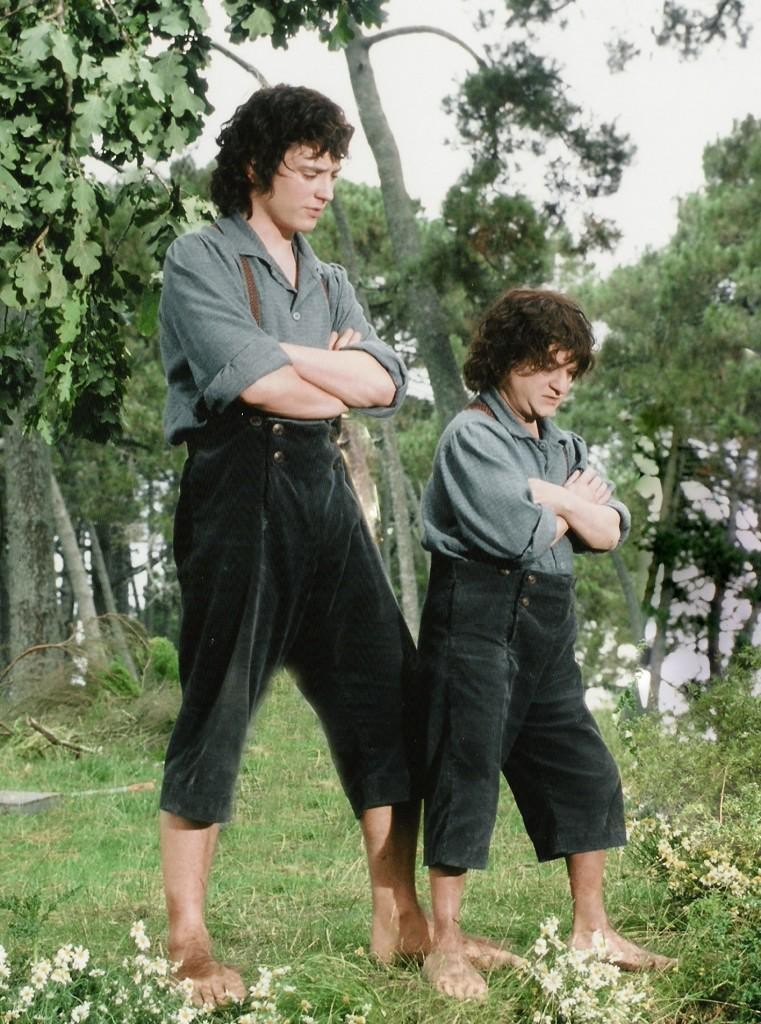
\includegraphics[scale=0.1]{frodo1}
%\end{flushright}
%\end{minipage}  

\begin{columns}
    \begin{column}{0.7\textwidth}
\textsf{FrodoKEM} has a number of design options we cover:

\begin{itemize}
\item<.-> Both sets of parameters; 
\begin{itemize}

\item $\textsf{FrodoKEM-640}$ aims to match AES-128 security.

\item $\textsf{FrodoKEM-976}$ aims to match AES-192 security.
\end{itemize}

\item PRNG from AES and cSHAKE modules.

\item We focus on \textsf{FrodoKEM}, rather than the previous key exchange scheme \textsf{FrodoCCS} \cite{DBLP:conf/ccs/BosCDMNNRS16}.

\end{itemize}
    \end{column}
    \begin{column}{0.3\textwidth}
        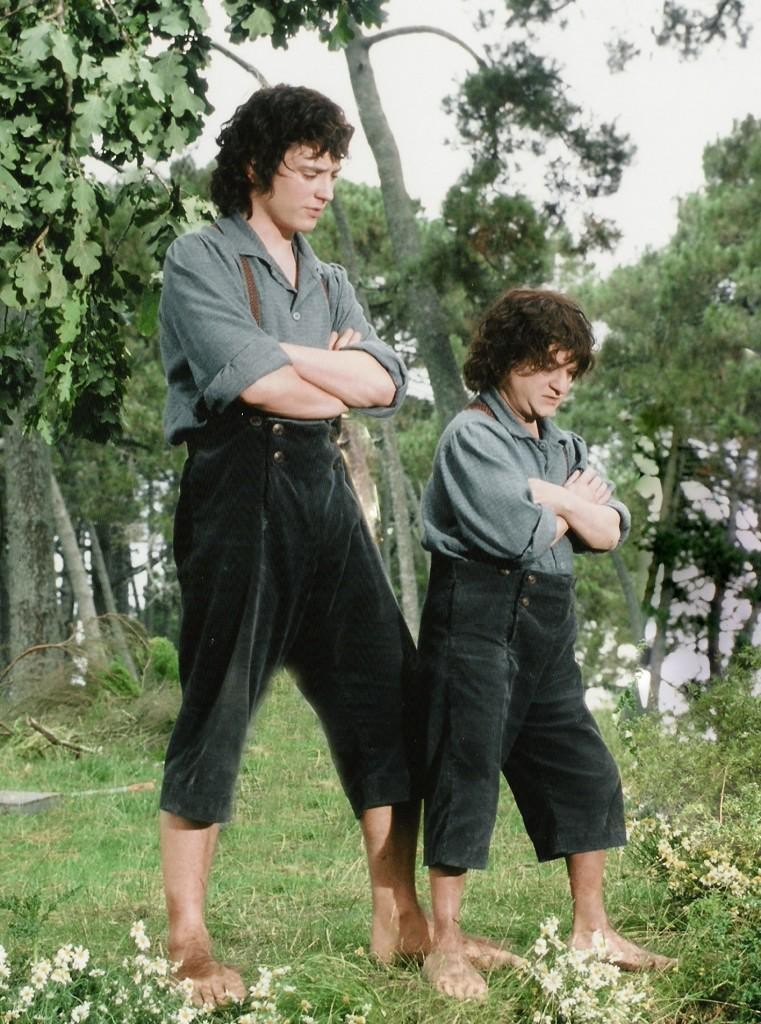
\includegraphics[scale=0.1]{frodo1}
    \end{column}
\end{columns}

\end{frame}

%%%%%%%%%%%%%%%%%%%%%%%%%%%%%%%%%%%%%%%%%%%%%%%%%%%%%%%%%%%%

\begin{frame}{FrodoKEM on ARM}

Contribution overview:

\begin{itemize}
\item Optimized memory allocation that makes the implementation small enough to fit on embedded microcontrollers.

\item An assembly multiplication routine that speeds up our implementation, realizing a performance that fits the requirements of common use-cases.

\item Utilises constant runtime to protect against simple side-channel analysis.

\item \textsf{FrodoKEM-640} has a total execution time of 836 ms.

\end{itemize}
\end{frame}

%%%%%%%%%%%%%%%%%%%%%%%%%%%%%%%%%%%%%%%%%%%%%%%%%%%%%%%%%%%%

\begin{frame}{FrodoKEM on ARM}

\begin{columns}
\hspace{.5cm}
	\begin{column}{0.45\textwidth}
		\begin{figure}
		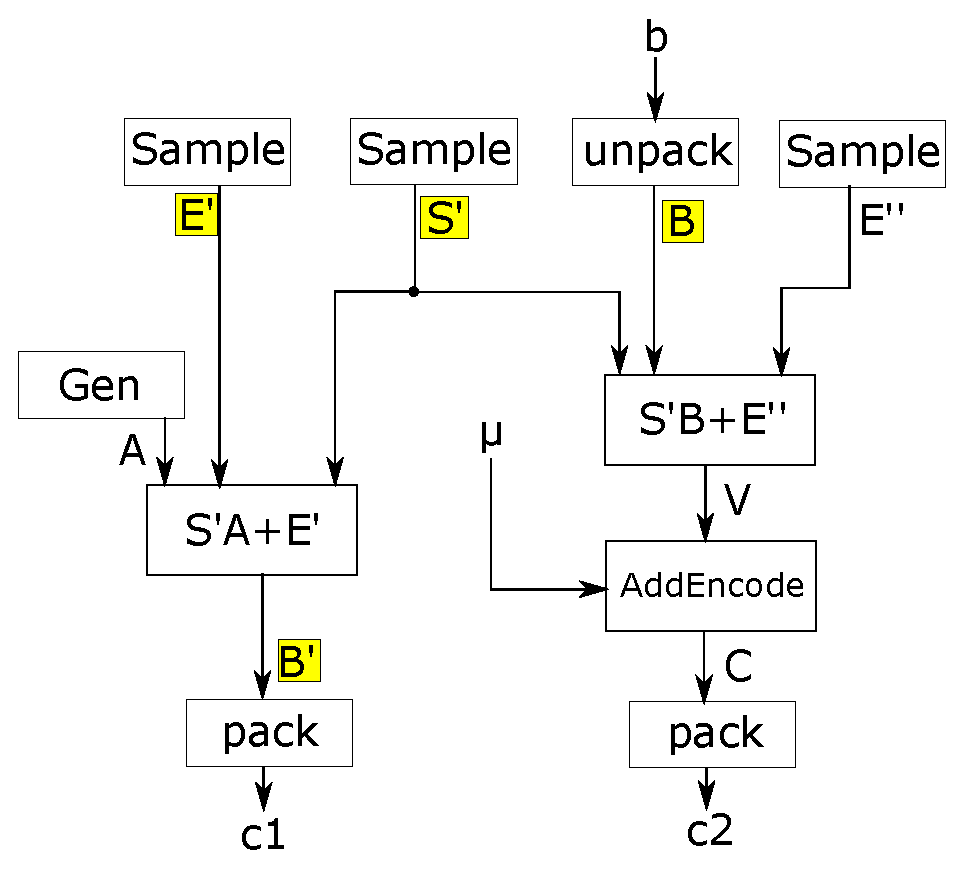
\includegraphics[scale=0.33]{frodo_flowchart_encaps}
		\caption{Flowchart of the encapsulation.}
		\end{figure}
    \end{column}
    \begin{column}{0.55\textwidth}
    \hspace{-3.5cm}
		\begin{itemize}
		\item We analysed the memory occupancy during each operation.
		\item Reusing already allocated memory wherever possible to 
		\item Minimizing the memory usage for all designs.		
		
		\end{itemize}
    \end{column}
\end{columns}

\end{frame}

%%%%%%%%%%%%%%%%%%%%%%%%%%%%%%%%%%%%%%%%%%%%%%%%%%%%%%%%%%%%

\begin{frame}{Results and Comparisons}

\begin{itemize}
\item Clear difference between AES and cSHAKE implementations.

\item Outperforms other Frodo design, but much slower than Kyber / NewHope.

%\item Utilises constant runtime in order to protect against simple side-channel analysis.

\end{itemize}

\begin{table}[tbhp]
%\footnotesize
\centering
\caption{\footnotesize Cycle counts for our full microcontroller implementations (at 168 MHz).}
\resizebox{0.65\textwidth}{!}{
\noindent\makebox[\textwidth]{
\begin{tabular}{|c|c|c|c|}
\hline
Implementation & Platform & Security Level & Cycle counts\\\hline
\textsf{FrodoKEM-640-AES} 	& Cortex-M4 & 128 bits  & 140,398,055\\
\textsf{FrodoKEM-976-AES} 	& Cortex-M4 & 192 bits  & 315,600,317\\
\textsf{FrodoKEM-640-cSHAKE}	& Cortex-M4 & 128 bits  & 310,131,435\\
\textsf{FrodoKEM-976-cSHAKE} 	& Cortex-M4 & 192 bits  & 695,001,098\\ \hline \hline
\textsf{FrodoKEM-640-cSHAKE} \cite{pqm4} & Cortex-M4 & 128 bits & 318,037,129 \\ \hline
\textsf{KyberNIST-768} \cite{pqm4} & Cortex-M4 & 192 bits & 4,224,704 \\
\textsf{NewHopeUSENIX-1024} \cite{alkim2016newhope}	& Cortex-M4 &255 bits & 2,561,438 \\ \hline
ECDH scalar multiplication \cite{DBLP:journals/dcc/DullHHHPSS15} &  Cortex-M0 & pre-quantum & 3,589,850\\
\hline
\end{tabular}}}
%\vspace{-0.7cm}
\end{table}

\end{frame}

%%%%%%%%%%%%%%%%%%%%%%%%%%%%%%%%%%%%%%%%%%%%%%%%%%%%%%%%%%%%

\begin{frame}{Results and Comparisons}

\begin{itemize}
\item Despite being slower, cSHAKE requires less memory than AES.

\item Our memory optimisations save between 30-40\% compared to PQM4.

\item Versus the referenced designs we also save 66\% in peak stack usage.

\end{itemize}

\begin{table}[tbhp]
\centering
\caption{\footnotesize Stack usage in bytes for our microcontroller implementations.}
\resizebox{0.65\textwidth}{!}{
\noindent\makebox[\textwidth]{\label{tab:res_micro_mem}
\begin{tabular}{|l|c|c|c|c|c|c|}
\hline
& \multicolumn{2}{c|}{\textsf{FrodoKEM-AES}} &\multicolumn{2}{c|}{\textsf{FrodoKEM-cSHAKE}} &\multicolumn{2}{c|}{\textsf{FrodoKEM-cSHAKE} \cite{pqm4}} \\
Operation	  & $n=640$ & $n=976$ & $n=640$ & $n=976$ & $n=640$ & \% Savings \\
\hline
Keypair							& 23,396   & 35,484  & 22,376  & 33,800 & 36,536 & 39\% \\
Encaps							& 41,292   & 63,484  & 37,792  & 57,968 & 58,328 & 35\% \\
Decaps							& 51,684   & 63,628  & 48,184  & 58,112 & 68,680 & 30\% \\
\hline
\end{tabular}}}
\end{table}

\end{frame}

%%%%%%%%%%%%%%%%%%%%%%%%%%%%%%%%%%%%%%%%%%%%%%%%%%%%%%%%%%%%

\begin{frame}{FrodoKEM on FPGA}

Contribution overview:

%Our FPGA design targets a balance between area consumption and throughput performance. This design choice is seen in the limited use of one multiplier module and minimal use of memory. A LWE multiplication core is proposed which is constantly reused for the main operations of the scheme, where the remaining operations are computed in parallel, essentially making multiplication the critical path of the design. The runtime of this depends exactly on the number of inputs, meaning all designs run in constant time. Most designs utilize less than 2000 FPGA slices and can output 51 operations per second (20 ms) for the main parameter set and 22 operations per second (45 ms) for the higher parameter set.

\begin{itemize}
\item Proposes a generic LWE multiplication core which computes vector-matrix multiplication and error addition.
\item Generates future random values in parallel, minimising delays between vector-matrix multiplications.
\item Hybrid pre-calculated / on-the-fly memory management is used, which continuously updates previous values.
\item Ensures constant runtime by parallelising other modules with multiplication.
\item \textsf{FrodoKEM-640} has a total execution time of 60 ms.

%\item \textsf{FrodoKEM-640} takes 266 ms for key generation, 284 ms for encapsulation, 286 ms for decapsulation, resulting in a total execution time of 836 ms for a full run of the protocol.

\end{itemize}
\end{frame}

%%%%%%%%%%%%%%%%%%%%%%%%%%%%%%%%%%%%%%%%%%%%%%%%%%%%%%%%%%%%

\begin{frame}{FrodoKEM on FPGA}

\begin{figure}
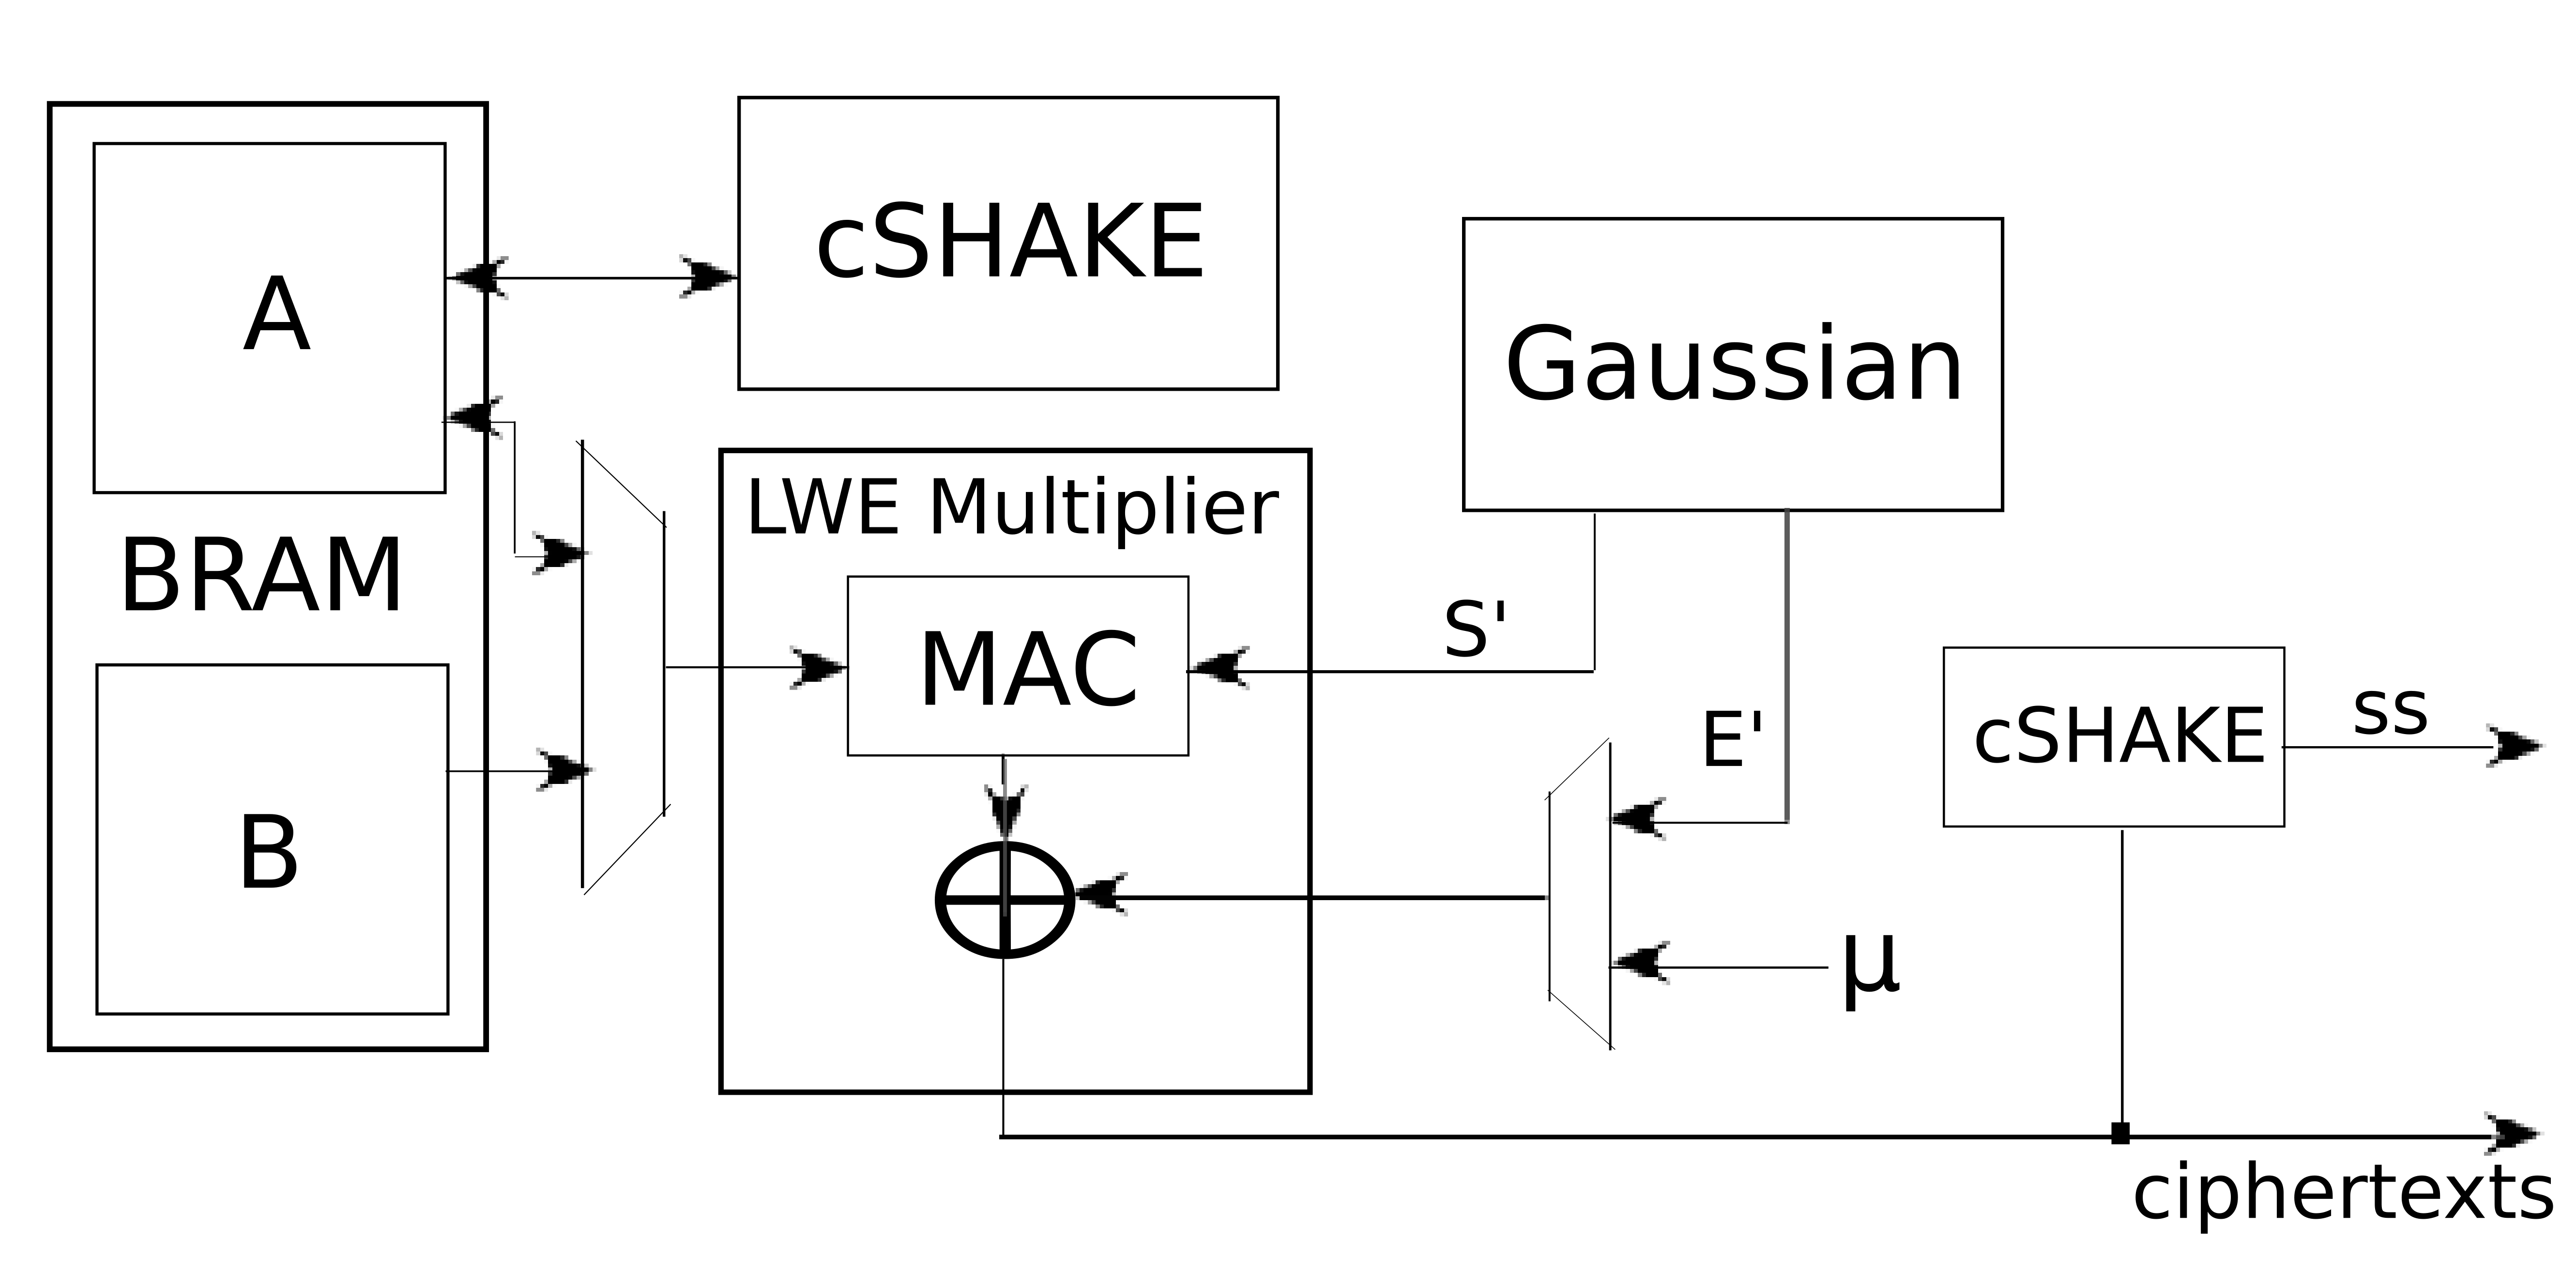
\includegraphics[scale=0.5]{FPGA_encaps}
\caption{An overview of our FPGA design of \textsf{FrodoKEM} Encapsulation.}
\end{figure}

\end{frame}

%%%%%%%%%%%%%%%%%%%%%%%%%%%%%%%%%%%%%%%%%%%%%%%%%%%%%%%%%%%%

%\begin{frame}{FrodoKEM on FPGA}
%DUMMY SLIDE
%\begin{itemize}
%%\item LWE multiplication is the critical path of all the proposed designs.
%
%\item The call suggests future rounds will likely involve:
%\begin{itemize}
%\item<.-> Evaluations on constrained devices, such as smart cards,
%\item<.-> as well as comparisons of the schemes in hardware.
%\end{itemize}
%\end{itemize}
%
%\begin{minipage}{0.55\textwidth}
%\begin{itemize}
%
%\item Why focus on lattice-based / Frodo?
%\begin{itemize}
%\item<.-> Extremely versatile and 
%\item<.-> Probably the most secure 
%\item<.-> Less implementations than ideal lattice schemes; has larger keys 
%\item<.-> Frodo is ideal for long-term security \emph{and} constrained 
%\end{itemize}
%
%\end{itemize}
%
%\end{minipage}
%\begin{minipage}{0.35\textwidth}
%\begin{flushright}
%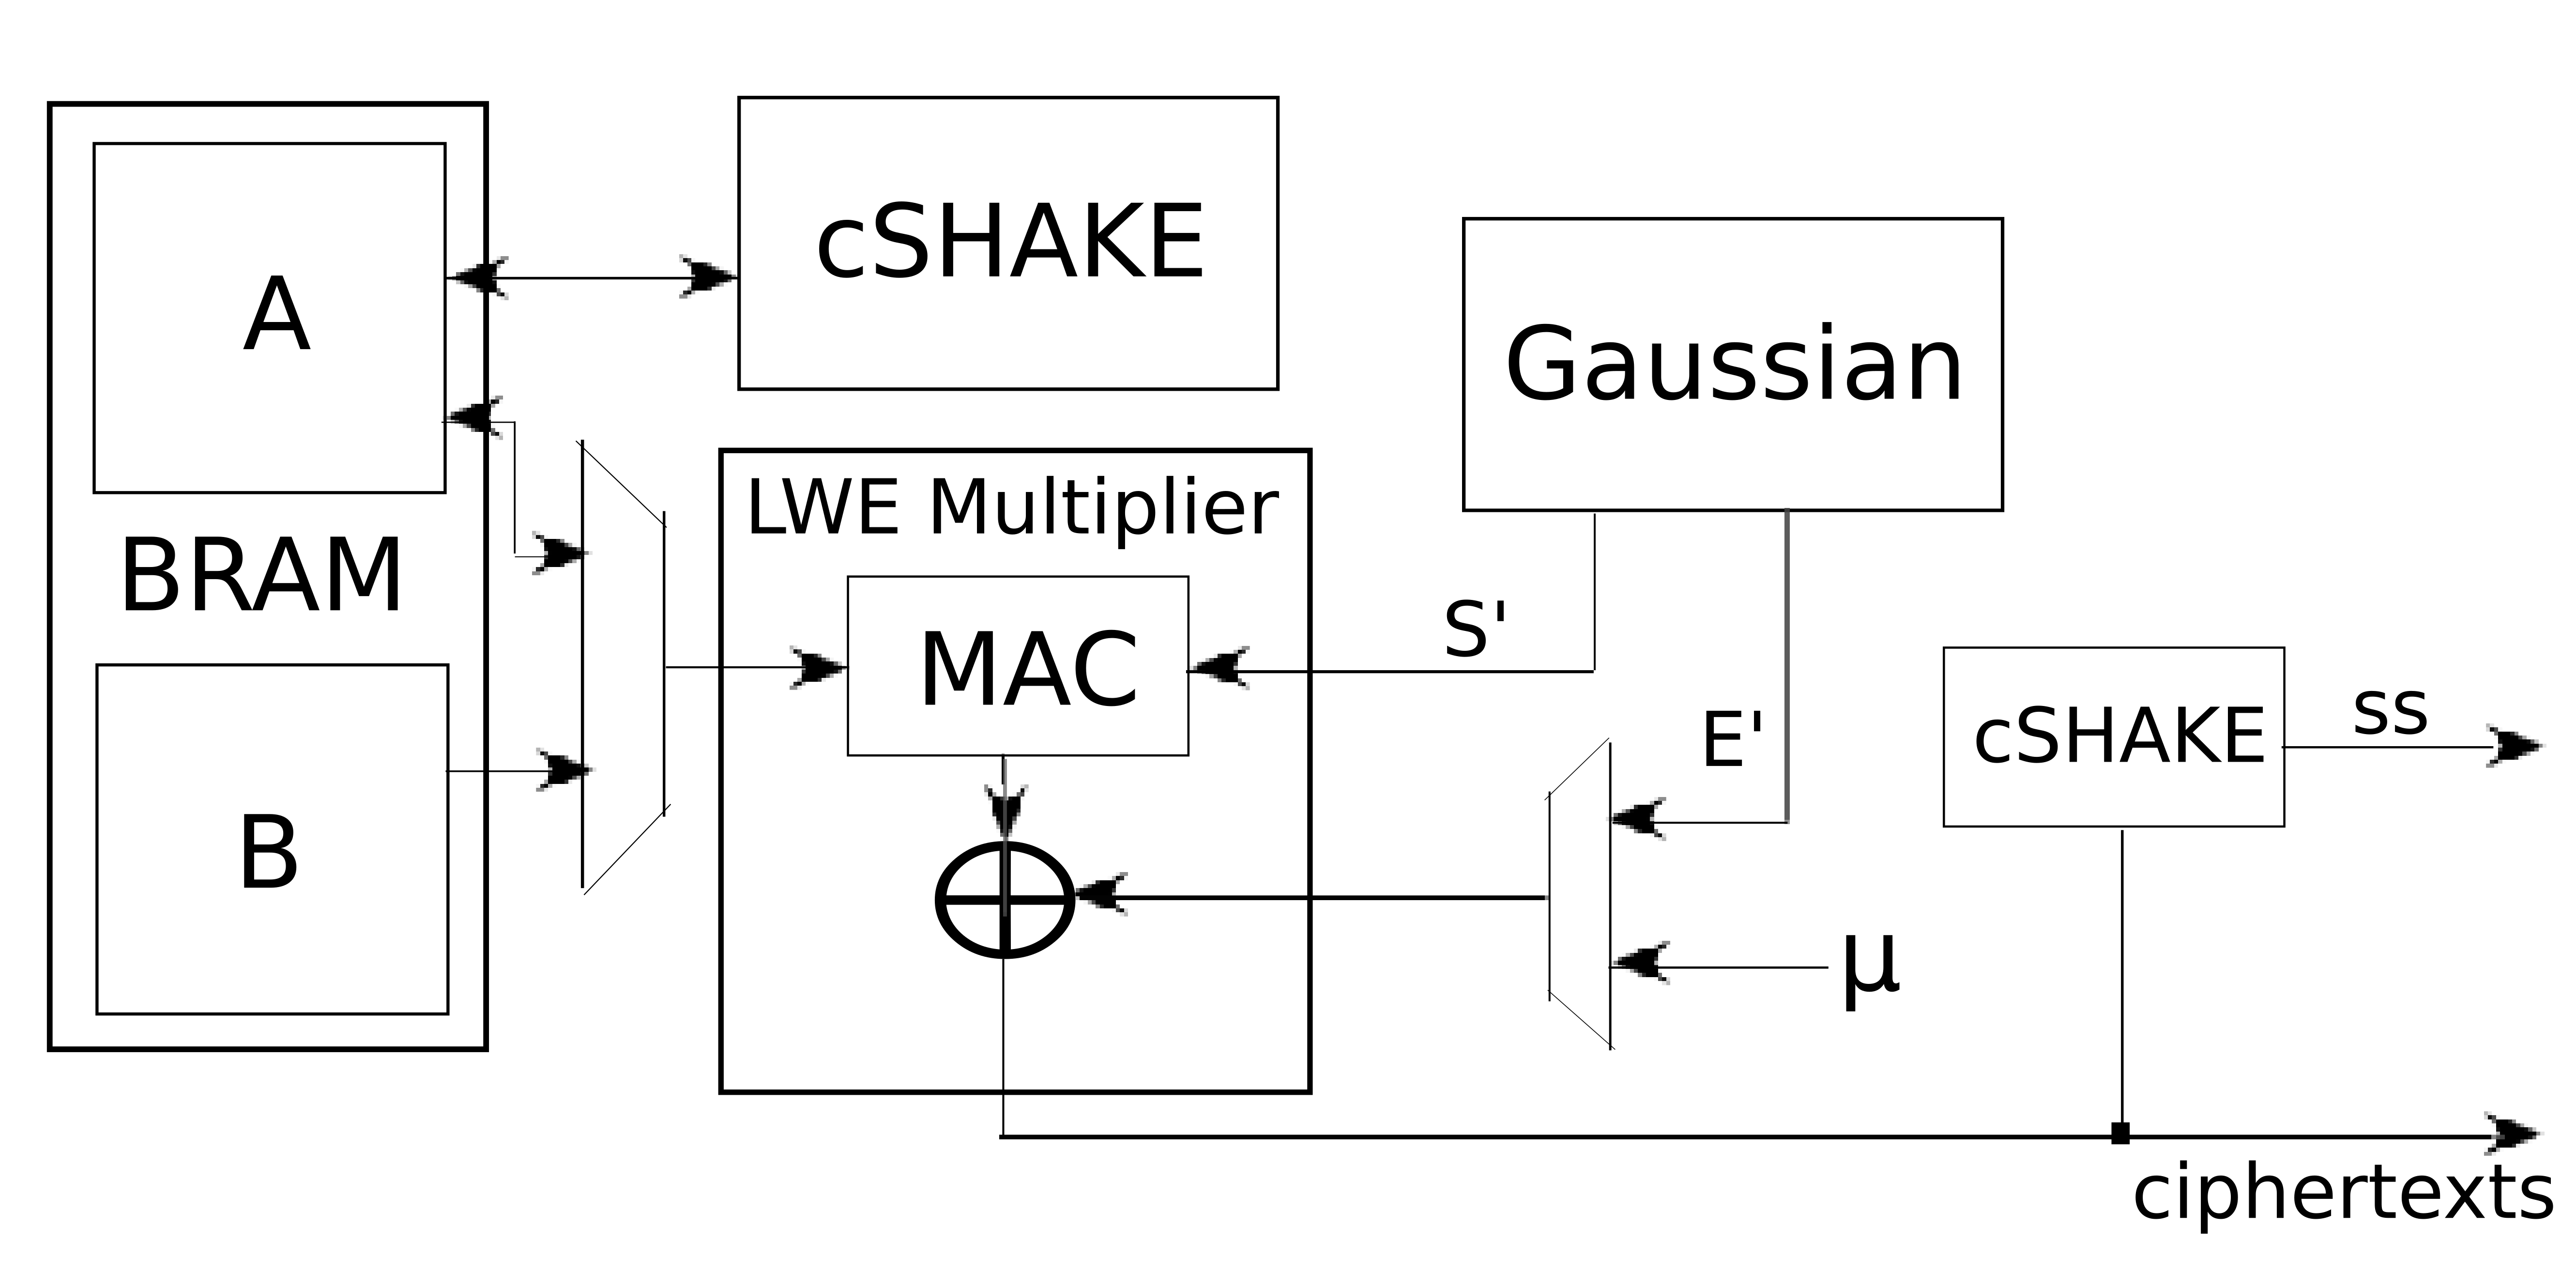
\includegraphics[scale=0.3]{FPGA_encaps}
%\end{flushright}
%\end{minipage}  
%
%
%
%%\item \textsf{FrodoKEM-640} takes 266 ms for key generation, 284 ms for encapsulation, 286 ms for decapsulation, resulting in a total execution time of 836 ms for a full run of the protocol.
%
%\end{frame}

%%%%%%%%%%%%%%%%%%%%%%%%%%%%%%%%%%%%%%%%%%%%%%%%%%%%%%%%%%%%


\begin{frame}{Results and Comparisons}

\begin{itemize}
\item Competes with NewHope area consumption, but much slower performance.
\item Huge savings in BRAM compared to LWE Encryption \cite{DBLP:conf/dac/HoweMORGB16}.
\end{itemize}
\vspace{-0.3cm}
\begin{table}[tbhp]
\caption{\footnotesize FPGA consumption and performance of our proposed designs, benchmarked on Artix-7.}
\begin{center}
\resizebox{0.65\textwidth}{!}{
\noindent\makebox[\textwidth]{
\begin{tabular}{|c|c|c|c|c|c|c|}
\hline
%& \multicolumn{2}{c|}{\textsf{FrodoKEM-AES}} &\multicolumn{2}{c|}{\textsf{FrodoKEM-cSHAKE}} &&\\
\textbf{Cryptographic Operation}& \textbf{LUT/FF} & \textbf{Slice} & \textbf{DSP} & \textbf{BRAM} & \textbf{MHz} & \textbf{Ops/sec}\\
\hline
\textsf{FrodoKEM-640} Keypair 	& 6621/3511 & 1845 & 1 & 6  & 167 & 51 \\
\textsf{FrodoKEM-640} Encaps	& 6745/3528 & 1855 & 1 & 11 & 167 & 51 \\
\textsf{FrodoKEM-640} Decaps	& 7220/3549 & 1992 & 1 & 16 & 162 & 49 \\ \hline
\textsf{FrodoKEM-976} Keypair	& 7155/3528 & 1981 & 1 & 8  & 167 & 22 \\
\textsf{FrodoKEM-976} Encaps	& 7209/3537 & 1985 & 1 & 16 & 167 & 22 \\
\textsf{FrodoKEM-976} Decaps	& 7773/3559 & 2158 & 1 & 24 & 162 & 21 \\ \hline
cSHAKE$^*$	& 2744/1685 & 766 & 0 & 0 & 172 & 1.2m \\
Error+AES Sampler$^*$ & 1901/1140 & 756 & 0 & 0 & 184 & 184m \\

\hline\hline
\textsf{NewHopeUSENIX} Server \cite{oder2017implementing} 	& 5142/4452 & 1708 & 2 & 4 & 125 & 731 \\
\textsf{NewHopeUSENIX} Client \cite{oder2017implementing}	& 4498/4635 & 1483 & 2 & 4 & 117 & 653 \\ \hline
\textsf{LWE} Encryption \cite{DBLP:conf/dac/HoweMORGB16}    & 6078/4676 & 1811 & 1 & 73 & 125 & 1272 \\
\hline
\end{tabular}}}
\end{center}
\end{table}

\end{frame}

%%%%%%%%%%%%%%%%%%%%%%%%%%%%%%%%%%%%%%%%%%%%%%%%%%%%%%%%%%%%

\begin{frame}{Conclusions}

\begin{itemize}
%\item Our results show the efficiency of \textsf{FrodoKEM} on embedded devices, a possible future post-quantum standard.

\item We show that hardware significantly minimises the performance distance between standard and ideal lattice-based KEM, able to utilise less than 2000 slices and remain practical.

\item Memory optimisations for microcontrollers show 66\% savings vs reference design and 40\% vs optimised PQM4 design.

%\item FrodoKEM is 

\end{itemize}

\end{frame}

%%%%%%%%%%%%%%%%%%%%%%%%%%%%%%%%%%%%%%%%%%%%%%%%%%%%%%%%%%%%

\begin{frame}{Conclusions}


\begin{itemize}
\item Our results show the efficiency of \textsf{FrodoKEM} and help to assess the practical performance of a possible future post-quantum standard.

%\vspace{0.5cm}
\end{itemize}

\begin{center}
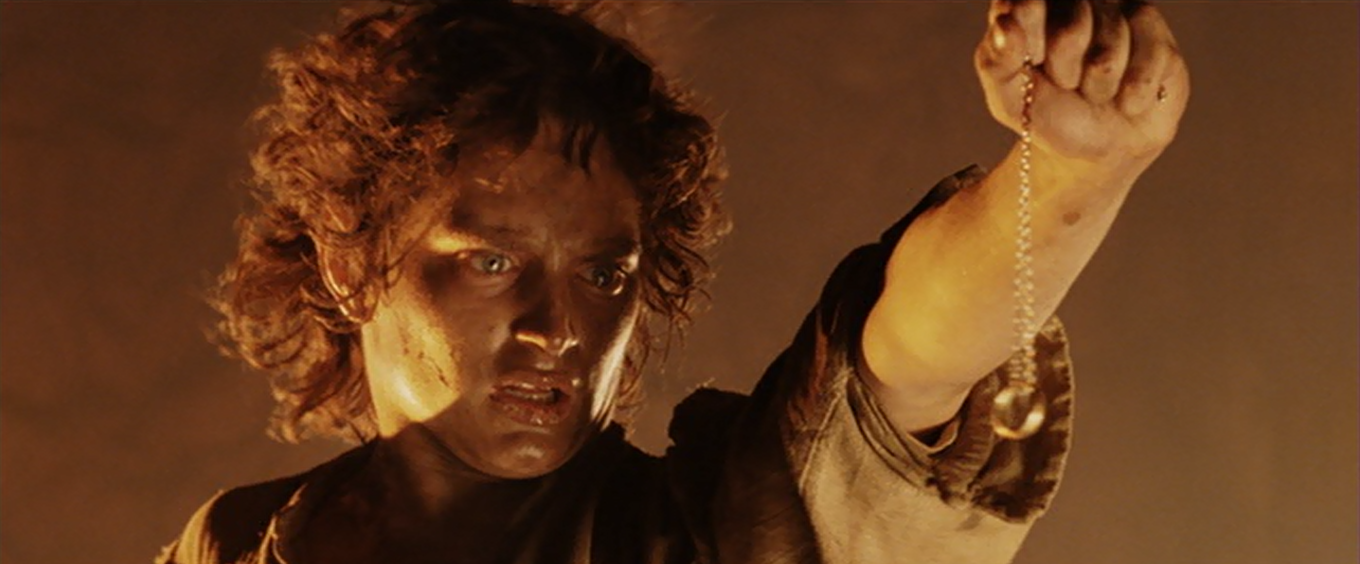
\includegraphics[scale=0.15]{Frodo_Doom}
\end{center}

\end{frame}

%%%%%%%%%%%%%%%%%%%%%%%%%%%%%%%%%%%%%%%%%%%%%%%%%%%%%%%%%%%%
\begin{frame}

\begin{center}
Although rings are still good to use, unless you're Gollum...\vspace{0.5cm}

\animategraphics[loop,autoplay,width=.7\linewidth]{5}{gollum/727f4870d47c42dbfe564b92f35209e0-}{0}{56} %727f4870d47c42dbfe564b92f35209e0-37

\vspace{0.5cm}

Thank you for listening. Any questions?

\end{center}

\end{frame}


\begin{frame}[allowframebreaks]{References}\scriptsize
\bibliographystyle{alpha}
\bibliography{paper.bib}
\end{frame}

%%%%%%%%%%%%%%%%%%%%%%%%%%%%%%%%%%%%%%%%%%%%%%%%%%%%%%%%%%%%
\end{document}

%%%%%%%%%%%%%%%%%%%%%%%%%%%%%%%%%%%%%%%%%%%%%%%%%%%%%%%%%%%%%%%%%%%%%%%%%%%%%%
